\chapter{Algoritmul de recomandare }
\label{chap:ch1}

\section{Prelucrarea datelor}
\label{sec:ch3sec1}
\par Un prim pas in algoritmul de recomandare de filme este de a prelucra datele pentru a obtine cele mai bune valori in calculul final al scorului. Dupa ce avem toate datele un prim pas este sa inlocuim datele nule cu caracterul spatiu pentru a nu conta in calculul final. Apoi un pas destul de important in procesarea datelor este sa eliminam cuvintele de legatura ca de exmplu:  ‘an’, ‘be’, ‘some’, etc.  Cel mai important camp din care trebuie scoase aceste cuvinte este descrierea deoarece la final se vor crea vectori din cuvintele pe care le avem in datele noastre, iar cuvintele de legatura nu sunt deloc importante in calculul final noi avand nevoie doar de cuvintele estentiale. Ultimul lucru care trebuie facut in procesarea datelor este de a scoate separatorii de cuvinde, in datele noastre fiind doar virgula, din colonele:gen, actori, scriitori, directori si descriere. 

\section{Sacul de cuvinte si transformrea cuvintelor in vectori }
\par Urmatorul pas in algorituml de recomandare de filme este de a creaa cea ce se numeste “Bag of words”. Modelul “Bag of words” este o reprezentare pentru procesarea limbajului natural și regăsirea informațiilor care simplifică lucrurile (IR). Un text (cum ar fi o propoziție sau un document) este reprezentat în această paradigmă ca un sac (multiset) al cuvintelor sale, care ignoră sintaxa și chiar ordinea cuvintelor, păstrând în același timp multiplicitatea. Viziunea computerizată a utilizat, de asemenea, conceptul de sac de cuvinte. Pentru a creea sacul de cuvinte se lipesc toate toate datele de care avem nevoie in calculul scorului final: descrierea fara cuvinte de legatura,gen, actori, scriitori, directori si descriere, intr-un singur camp pe care il numin “bag” aceasta operatie facandu-se pentru fiecare film, deci fiecare film va avea propiul bag. Urmatorul pas este de a pune toate bag-urile la un loc si de a scoate duplicatele la urma ramanand cu n cuvinte care apar in datele din toate filmele.  Pe baza acestor cuvinte se va creea pentru fiecare film cate un vector de dimensiune n fiecare pozitie reprezentand frecventa cuvantului din filmul curent. Ca exeplu pentru explicatia de mai sus luam trei propozitii: 
		\begin{figure}[htbp]
			\centerline{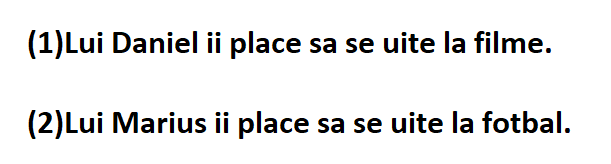
\includegraphics[width=16cm, height=4cm]{figures/cele 2 poze.png}}
			\caption{Propozitii pentru exemplu}
			\label{fig}
		\end{figure}
\par Dupa ce scoatem cuvintele de legatura:lui, ii, sa, se, propozitiile prima propozitie va arata Daniel, place, uite, filme , iar a doua Marius place uite fotbal. Dupa ce se lipesc cele doua propozitii campul cuvintelor va fi: Daniel, place, uite, filme, Marius, fotbal. Apoi vectori care se vor creea pentru cele doua propozitii vor arata in felul urmator: 

		\begin{figure}[htbp]
			\centerline{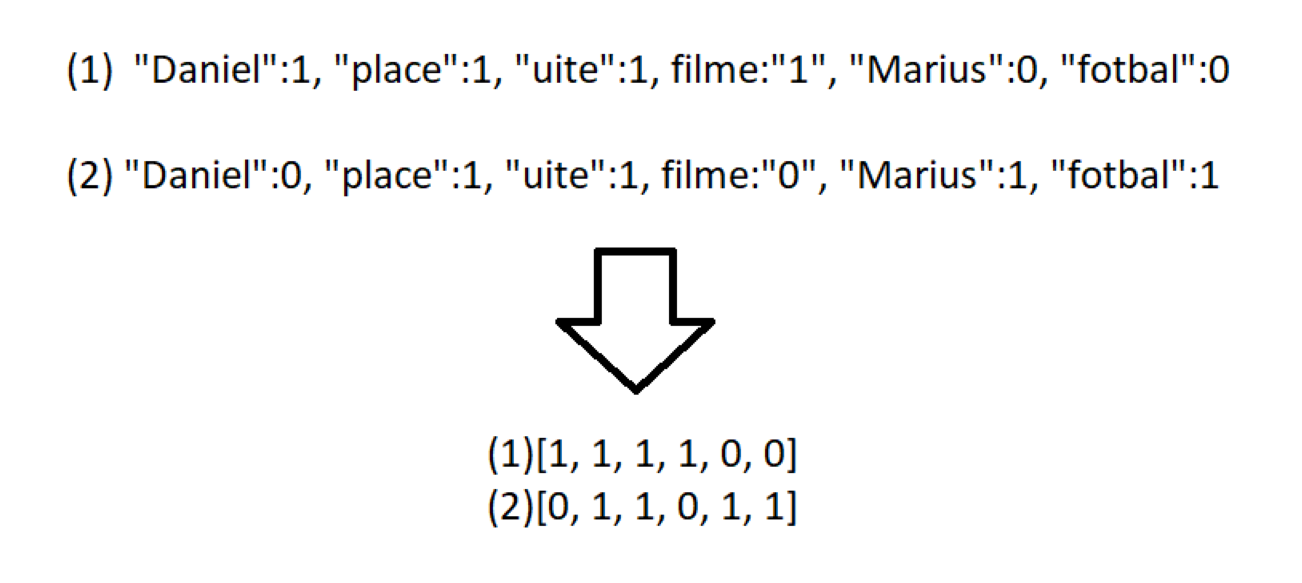
\includegraphics[width=16cm, height=9cm]{figures/rezultat vectori.png}}
			\caption{Propozitii pentru exemplu}
			\label{fig}
		\end{figure}

\section{Similaritatea cosinus }
\par Metrica de similaritate cosinus este utilizată pentru a determina cât de asemănătoare sunt documentele, indiferent de mărimea lor. Aceasta estimează matematic cosinusul unghiului format de doi vectori proiectați într-un spațiu multidimensional. Similaritatea cosinusului este utilă deoarece, chiar dacă două documente comparabile sunt separate de o distanță euclidiană mare (din cauza dimensiunii documentelor), este probabil ca acestea să fie similare. Pentru acest model, se foloseste similaritatea cosinusului pentru a defini "similitudinea" dintre filme.Motivul pentru care nu se folosește doar distanța dintre vectori ca scor de similaritate, chiar dacă ar putea părea rezonabil, lungimile vectorilor pot afecta distanța euclidiană, dar nu și distanța cosinus (1 - cos(unghi)). Deoarece lungimile a doi vectori definesc dimensiunea acestora (de exemplu, cantitatea de date), dar unghiul definește mai bine caracteristicile lor în lipsa unor cuvinte mai bune. Prin urmare, distanța unghiulară este mai potrivită pentru a defini similitudinea lor.
		\begin{figure}[htbp]
			\centerline{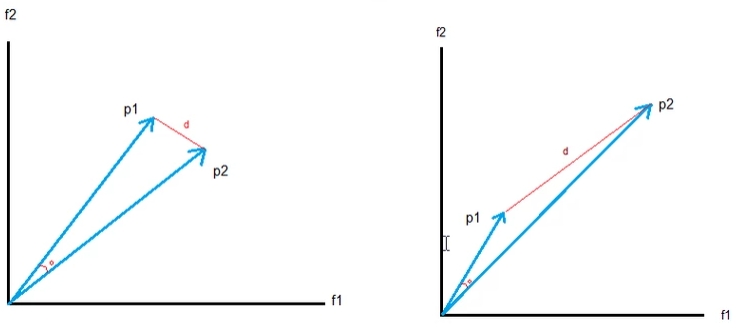
\includegraphics[width=12cm, height=5cm]{figures/grafic distanta.png}}
			\caption{Distanca euclidiana vs. distanta ungiulara}
			\label{fig}
		\end{figure}
\par După cum se poate  vedea, distanța euclidiană devine mult mai mare pe al doilea grafic, chiar dacă unghiul este destul de mic.

\section{Calcularea scorului final}
\par Dupa ce se calculeaza o matrice in care perechea (i,j) reprezinta similaritatea cosinus dintre doua filme se calculeaza inca o matrice care va reprezenta scorul final. Similaritatea cosinus va fi imbunatatita in functie de cat de apreciat este un film, astfel zece procente din scorul final le va reprezenta media dintre suma voturilor si numarul de votanti. La final se vor lua cele mai mari n scoruri , n reprezentand numarul de filme pe care vrem sa le recomandam, exceptandul pe primul deoarece cel mai bun scor il va avea filmul insusi.